\paragraph{Sơ đồ tuần tự luồng tạo chia sẻ cuộc trò chuyện}

Luồng nghiệp vụ này mô tả
vòng đời của một yêu cầu chia sẻ cuộc trò chuyện,
lưu trữ dữ liệu trò chuyện dưới dạng tệp tin JSONL trên Cloud Storage
và đồng bộ trạng thái giữa các dịch vụ thông qua mô hình
Transactional Outbox kết hợp Message Broker.

\begin{figure}[H]
\centering
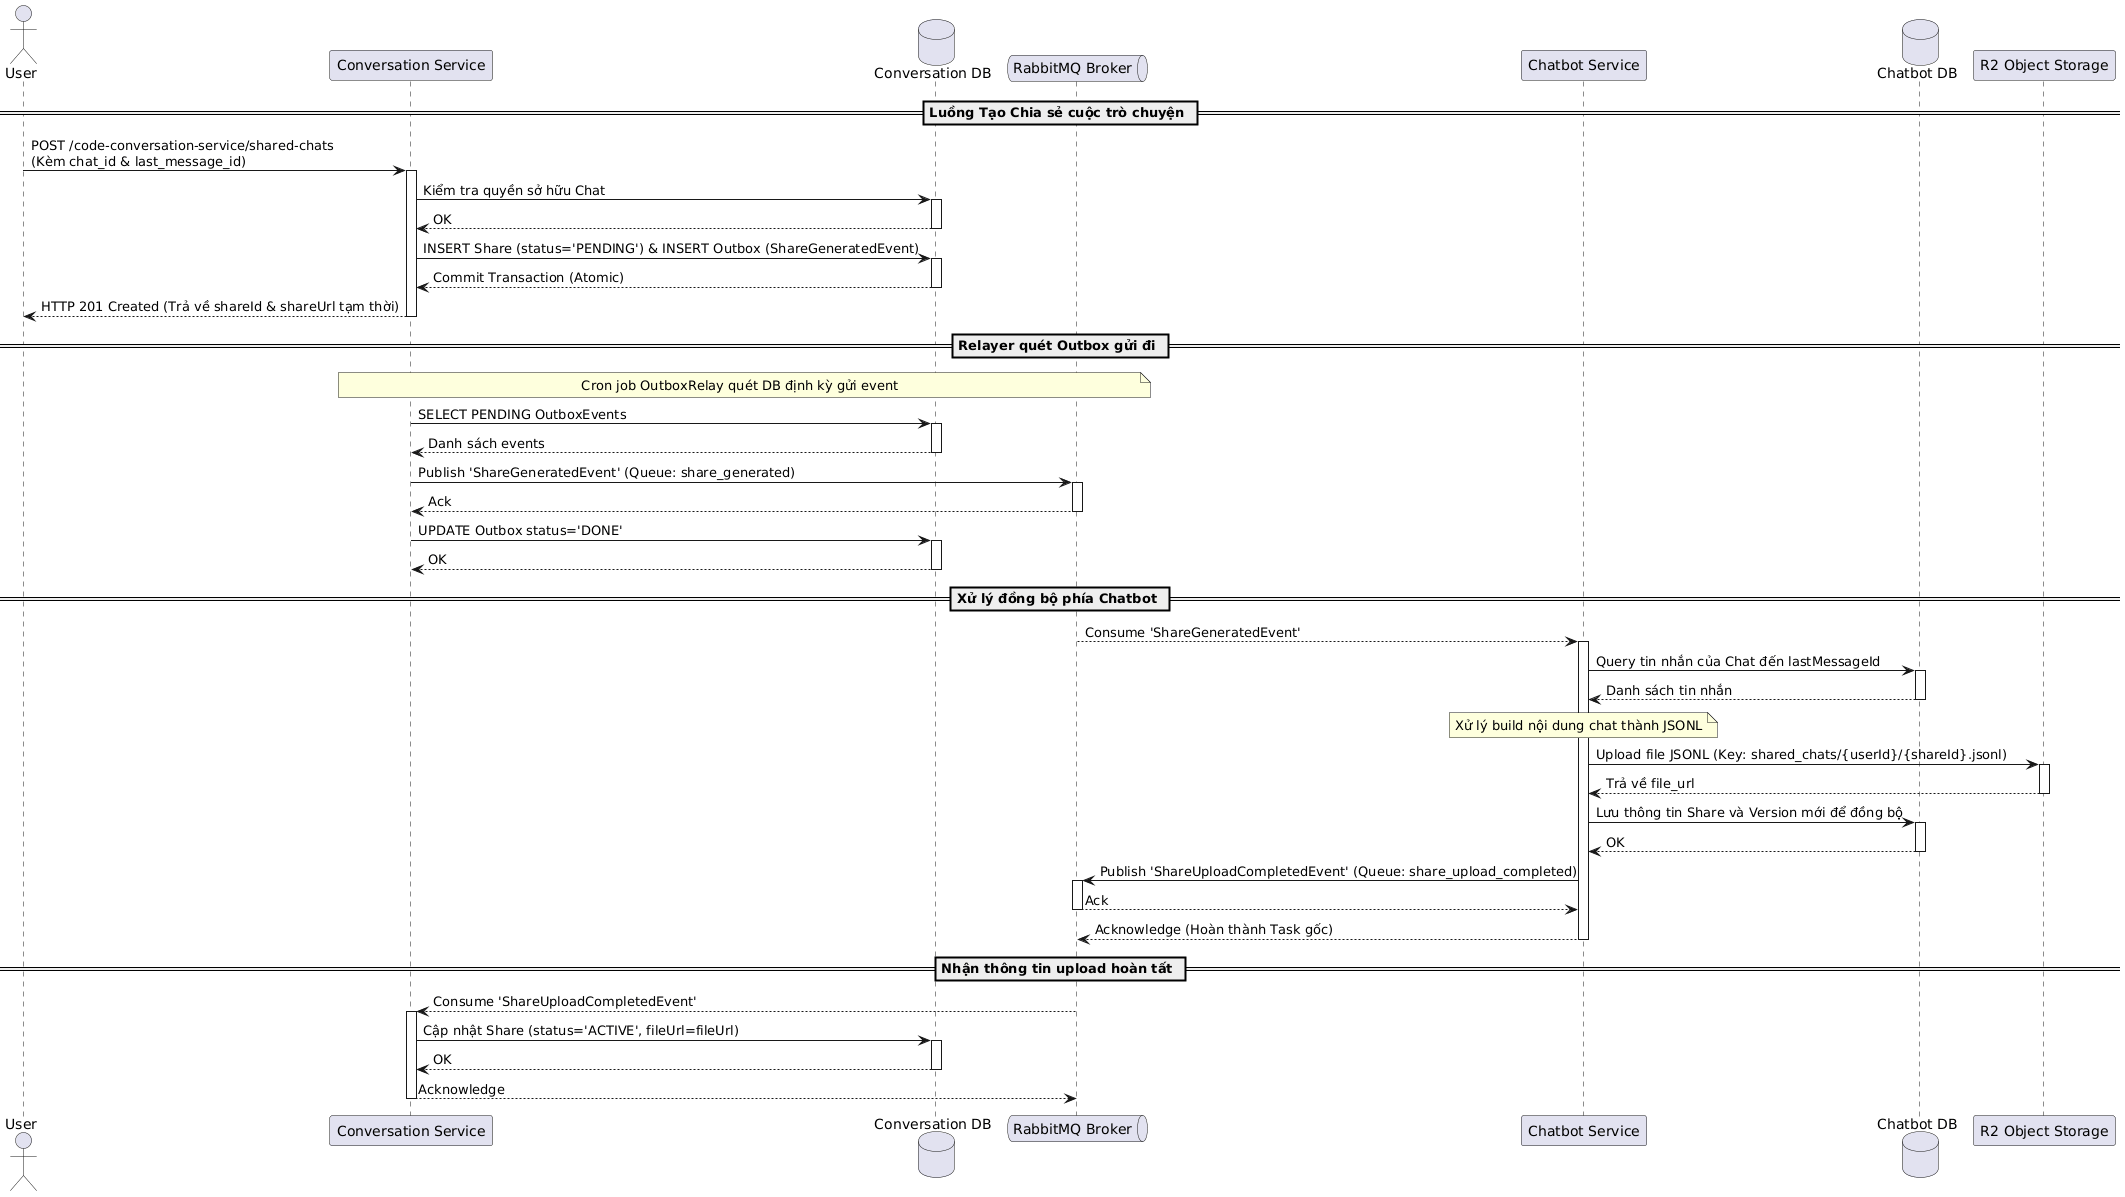
\includegraphics[width=0.95\textwidth]{contents/Sequence/UML-Sequence-UserCreateSharedChat.png}
\caption{Sơ đồ tuần tự luồng tạo chia sẻ cuộc trò chuyện}
\end{figure}

\begin{table}[H]
\centering
\renewcommand{\arraystretch}{1.3}

\begin{tabular}{|l|l|p{5cm}|}
\hline
\textbf{Thành phần} & \textbf{Phân loại} & \textbf{Vai trò trong hệ thống} \\ \hline
User & Actor & Người dùng gửi yêu cầu chia sẻ cuộc trò chuyện kèm theo tham số tin nhắn cuối để giới hạn phạm vi chia sẻ. \\ \hline
Conversation Service & Microservice & Dịch vụ quản lý tiếp nhận API từ người dùng, quản lý giao dịch Outbox và cập nhật trạng thái chia sẻ cuối cùng. \\ \hline
Conversation DB & Database & CSDL của Conversation Service, lưu trữ thông tin chung về trò chuyện, bản ghi chia sẻ và các sự kiện trong bảng Outbox. \\ \hline
RabbitMQ Broker & Message Broker & Message Broker nhận sự kiện và phân phối đến các dịch vụ theo dõi. \\ \hline
Chatbot Service & Microservice & Dịch vụ AI nhận sự kiện, trích xuất nội dung tin nhắn và tải lên file chia sẻ. \\ \hline
Chatbot DB & Database & CSDL lưu trữ lịch sử chi tiết của cuộc trò chuyện và thông tin chia sẻ. \\ \hline
R2 Object Storage & External Service & Hạ tầng lưu trữ đối tượng (Object Storage tương thích S3), sử dụng để lưu trữ tệp tin cấu trúc JSONL chứa nội dung chi tiết của cuộc trò chuyện được chia sẻ. \\ \hline
\end{tabular}
\caption{Các thành phần tham gia luồng tạo chia sẻ cuộc trò chuyện}
\end{table}

\subparagraph{Mô tả tổng quan}

\begin{itemize}

\item \textbf{Yêu cầu chia sẻ:}
Người dùng yêu cầu
chia sẻ cuộc trò chuyện
kèm định danh tin nhắn cuối cùng muốn chia sẻ.

\item \textbf{Khởi tạo bản ghi chia sẻ:}
Dịch vụ trò chuyện
tạo một bản ghi liên kết chia sẻ
ở trạng thái chờ xử lý
và lưu sự kiện chia sẻ vào bảng sự kiện chờ gửi
trong cùng một giao dịch CSDL
để đảm bảo tính đồng bộ dữ liệu.

\item \textbf{Phản hồi liên kết tạm thời:}
Dịch vụ phản hồi liên kết chia sẻ tạm thời
về cho giao diện ngay lập tức
để giảm thời gian chờ đợi của người dùng.

\item \textbf{Chuyển sự kiện tạo chia sẻ:}
Tiến trình quét bảng sự kiện định kỳ,
lấy ra các sự kiện chia sẻ chưa xử lý
và gửi sự kiện tạo chia sẻ vào hàng đợi tin nhắn.

\item \textbf{Truy vấn nội dung tin nhắn:}
Dịch vụ chatbot nhận sự kiện tạo chia sẻ từ hàng đợi,
truy vấn toàn bộ nội dung các tin nhắn trong cuộc trò chuyện tính
đến tin nhắn cuối cùng được yêu cầu chia sẻ từ CSDL chatbot.

\item \textbf{Tải dữ liệu lưu trữ:}
Dịch vụ chatbot đóng gói nội dung
cuộc trò chuyện thành tệp tin lưu trữ
và tải lên kho chứa trực tuyến, đồng thời cập nhật CSDL chatbot
và phát sự kiện đã hoàn tất tải tệp lên hàng đợi tin nhắn.

\item \textbf{Kích hoạt liên kết chính thức:}
Dịch vụ trò chuyện nhận sự kiện từ hàng đợi
và cập nhật trạng thái liên kết chia sẻ
thành đang hoạt động kèm theo đường dẫn tệp tin chính thức.

\end{itemize}
